\graphicspath{../assets}

\chapter{Modello}
\section{Lavori Precedenti e Considerazioni Generali}

La terminologia intelligenza artificiale, o alternativamente machine learngin,
indica un campo molto vasto che raccoglie molte e diverse tecniche di apprendimento
ed elabroazione dati, che possono spaziare su più livelli di complessità ed essere 
divisi in molteplici categorie.
Un primo distinguo che si puo' fare nel merito delle tecniche di apprendimento è quello
tra {\it shallow learning} e {\it deep learning}.
Il primo si potrebbe tradurre in italiano come "apprendimento superficiale",
mentre il secondo come "apprendimento profondo". \\
Seppure le differenze tra i due siano tante e non di poco conto, in entrambi i casi
abbiamo un algoritmo che dato un input $\vec{x}$, la cui realizzazione concreta
varia a seconda dell'approccio utilizzato e specifichieremo nel dettaglio quando
necessario, e ne calcolano un output $\vec{y} = f(\vec{x})$.
Anche per $\vec{y}$ la realizzazione concreta puo' differire molto, 
ma una forma generale è un vettore con $N_c$ dimensioni, $N_c$, dove $N_c$ è il numero di
classi del problema, ovvero il numero di possibili risposte.
Nel nostro specifico caso, dove cerchiamo soltanto di discriminare tra un tessuto
ritenuto sano ed uno ritenuto patologico, avremmo che $N_c = 2$.
Nel caso si stia trattando un problema binario come il nostro, un'altra alternativa
è quella di utilizzare un output di dimensione $N_c = 1$, che può essere un
vettore unidimensionale o uno scalare.


\begin{figure}
    \center
    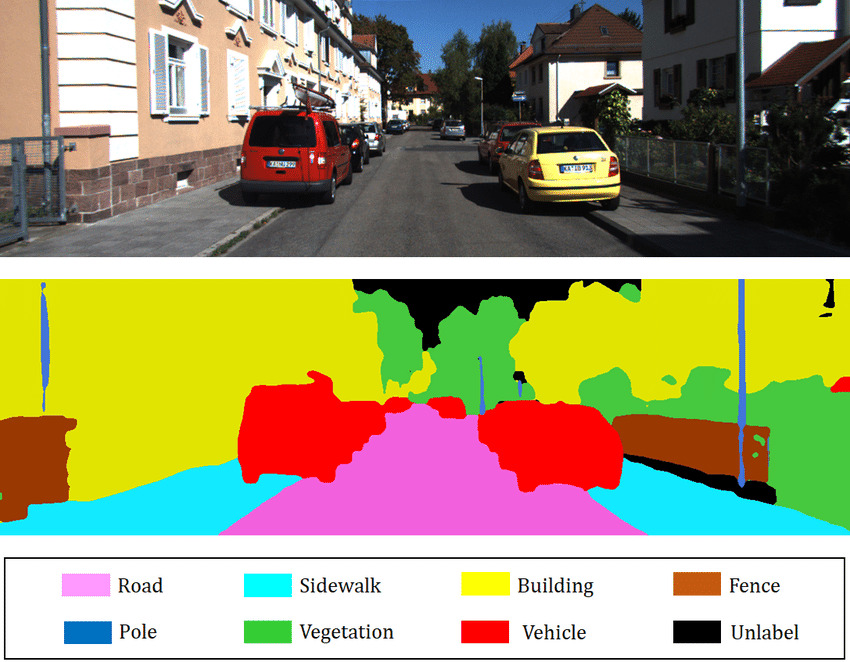
\includegraphics[width=0.9\textwidth]{./assets/semseg.jpg}
    \caption{\label{fig:semseg}Esempio di Semantic Segmentation applicata al riconoscimento di oggetti stradali. Fonte: https://towardsai.net/p/l/machine-learning-7}
\end{figure}

Il problema che si tenta di risolvere è denominato
{\it semantic segmentation}, di cui un esempio è visibile nella figura 
\ref{fig:semseg} un caso specifico della {\it image classification}.
Nella {\it image classification} infatti quel che si fa è dedurre cosa l'immagine
in input rappresenti, senza specificare quale parte dell'immagine contenga la classe
rilevata.
Nella {\it semantic segmentation} invece si vuole rilevare quale zona dell'immagine
contenga le classi rilevate. 
L'utilizzo del plurale nell'ultima frase non è casuale: se infatti nella {\it image classification}
un'immagine contnente più oggetti risponde generalmente con una sola classe,
nella {\it semantic segmentation} si gestisce anche il caso in cui siano presenti più
oggetti di diverse classi, come nel nostro caso in cui un'immagine contente un
tessuto potenzialmetne patologico conterrà anche parti di tessuto sano o
porzioni d'immagine che non rappresentano affatto dei tessuti.
Per questo motivo il nostro problema binario avrà come classi la classe $C_1$, che indicherà
le zone di tessuto ritenute come potenzialmente patologiche ({\it "sick"}) e la classe $C_0$,
che denomineremo {\it "sane"} in maniera impropria dato che comprenderà
anche la parte di sfondo dell'immagine.
Questo è dovuto al fatto che i dataset impiegati, spiegati nel dettaglio in 
\ref{sec:Dataset}, hanno la sola annotazione delle zone malate, e non distinguono tra
zone sane e sfondo.


\subsection{\label{sec:shallow-learning}Tecniche Shallow Learning: Alberi Decisionali}

Il nostro primo modello di riferimento\cite{Toma2022} è basato su
alberi decisionali, modelli molto popolari nel mondo del machine learning
per vari motivi, uno tra i quali è la capacità di poter interpretare il loro funzionamento.
Infatti se con modelli {\it deep learning} non è possibile, se non in
modo ristretto e con poche certezze, capire il processo di inferenza, 
gli alberi decisionali per costruzione sono molto
vicini al pensiero umano, e quindi facilmente interpretabili.
Modelli di questo tipo prendono anche il nome di modelli {\it white box},
mentre modelli non interpretabili prendono il nome di modelli {\it black box}.
Tuttavia, questa affermazione ha una validità relativa, in quanto
nel momento in cui i valori del campione in ingresso, vale a dire le
componenti del nostro vettore $\vec{x}$ salgono in numero e complessità,
interpretare il procedimento di inferenza diventa sempre più difficile non per
come il modello prende la decisione ma perché è difficile per le persone
valutare la decisione sulla base di valori statistici.

Il lavoro in questione non ha però semplicemente utilizzato degli decisionali,
ma piuttosto un {\it ensamble} di alberi decisionali, che prende il nome
di {\it random forest}, ovvero un insieme di un grande numero di alberi decisionali.
Questa è una metodologia molto diffusa sopratutto quando, per la difficoltà del
problema o per la scarsità dei dati, non si riesce a costruire un singolo
albero dai risultati soddisfacenti.
Quel che accade è che allora si utilizzano un numero elevati di alberi,
nel concetto generico qui descritti come {\it weak learners}, apprenditori
deboli, e ogni modello esprime la propria valtuazione sul campione.
Viene poi messo in atto un procedimento per ottenere un unico risultato finale,
che nel caso del lavoro descritto è il {\it majority vote}, dove si sceglie
il risultato che la maggioranza dei singoli alberi ha predetto.

\subsection{Algoritmo I}

Al fine di valutare i pro e i contro di questa metodologia, l'algoritmo
è stato reimplementato con alcune modifiche e lievi ottimizzazioni, assieme ad una
GUI per valutarne la praticità d'uso.

Come nel lavoro originale, l'immagine viene convertita in scala di grigi,
e si saltà il ritaglio delle immadini dal momento che esse sono già state
ritagliate in precedenza.
Dopodiché si applia comunque l'algoritmo di {\it K-Means} per rimuovere
i riflessi di luce.
In questo caso per velocizzare il processo si utilizza comunque un numero
$K=30$, con la differenza che non si utilizza un'inizializzazione
casuale ma si parte da una suffivisiione equispaziata da 0 a 255, ovvero
il massimo e il minimo valore di intensità dei pixel, oltre a iterare
il procedimento una sola volta.
Si rimuovono i pixel che ricadono nei tre cluster a intensità maggiore.
Infine si applica il metodo del gradiente di Sobel per evidenziare i bordi
e le discontinuità nelle venature del tessuto.
Dall'immagine ottenuta si estraggono delle {\it ROI} ({\it Region of Interest}),
anche dette {\it patches}, che sono delle porzioni dell'immagine di dimensione
fissa 50$\times$50 pixel, con una sovrapposizione del 40\% (20 pixel), ovvero
alcuni pezzi di una ROI fanno anche parte di altre ROI adiacenti.
Un esempio di questo tipo di sovrapposizione è mostrato in Figura \ref{fig:patch-overlap}.


Da qui vengono estratti i primi 11 valori statistici che andranno a comporre
i primi 11 valori del nostro vettore $\vec{x}$, che rappresenta la ROI in
ingresso.
A questi vengono poi agginti valori estratti da due matrici che vengono
calcolate dalla ROI stessa, la {\it Gray-Level Co-occurrence Matrix} (GLCM)
e la {\it Gray-Level Run Length Matrix} (GLRLM), che hanno prodotto
risultati soddisfacenti quando applicate ad altri problemi di
{\it pattern recognition}.\cite{GLCM}\\
In entrambi i casi bisogna anzitutto portare l'immagine da scala di grigi
a livelli di grigi.
Un'immagine bianco e nero è composta da un solo canale, con valori che possono
essere rappresentati come numeri interi tra 0 e 255.
Nel caso più generico potremmo dire che un'immagine in bianco e nero
è un'immagine che ha 256 livelli di grigi, ma questo non è ottimale al
funzionamento delle matrici, per cui si digitalizza l'immagine a un numero molto
minore di livelli di grigio, in questo caso 4.
Questo significa che, ai fini del calcolo delle matrici, i valori di grigio
dell'immagine tra 0 e 63, varrà 1 tra 64 e 127, e così via.\\
La GLCM è una matrice quadrata di dimensione $N \times N$, dove $N$ è il
numero di livelli di grigio, che contiene i valori di frequenza con cui
si ripetono coppie di pixel vicini.
È caratterizzata da due parametri, la {\it distanza} $d$ e l'{\it angolo} $\theta$,
ed è possibile utilizzarne molteplici per calcolare più matrici,
ma in questo caso è stata utilizzata una sola matrice, con $d=1$ e $\theta=0$°.
La distanza indica a che distanza cercare la co-occorrenza, nel caso di $d=1$
significa guardare l'elemento adiacente, mentre l'angolo indica la direzione
di adiacenza, in questo caso $0$° quello a destra dell'elemento considerato.

\begin{figure}[h]
    \center
    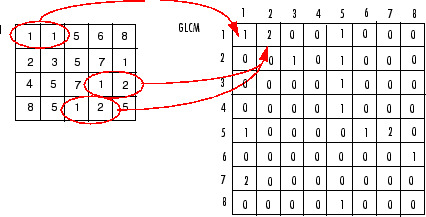
\includegraphics[width=0.9\textwidth]{./assets/glcm.jpg}
    \caption{Illustrazione del Calcolo di una GLCM a 8 livelli di grigio, fonte: https://it.mathworks.com/help/images/create-a-gray-level-co-occurrence-matrix.html}
\end{figure}

Da tale matrice si vanno ad estrarre altri 4 valori statistici.
Segue poi un processo simile per la GLRLM, anch'essa di dimensione
$N \times N$, dove $N$ è nuovamente il numero di livelli di grigio,
ma che è caratterizzata da un solo parametro, l'angolo $\theta$,
che indicia la direzione verso cui viene misurata una {\it run}.
In tale matrice, l'elemento $g_{i,j}$ rappresenta il numero di {\it run}
di lunghezza $j$ percorse nella direzione $\theta$ composte tutte dal medesimo
livello di grigio $i$.
Una rappresentazione visiva del calcolo è riportata nella Figura \ref{fig:glrlm}.

\begin{figure}
    \center
    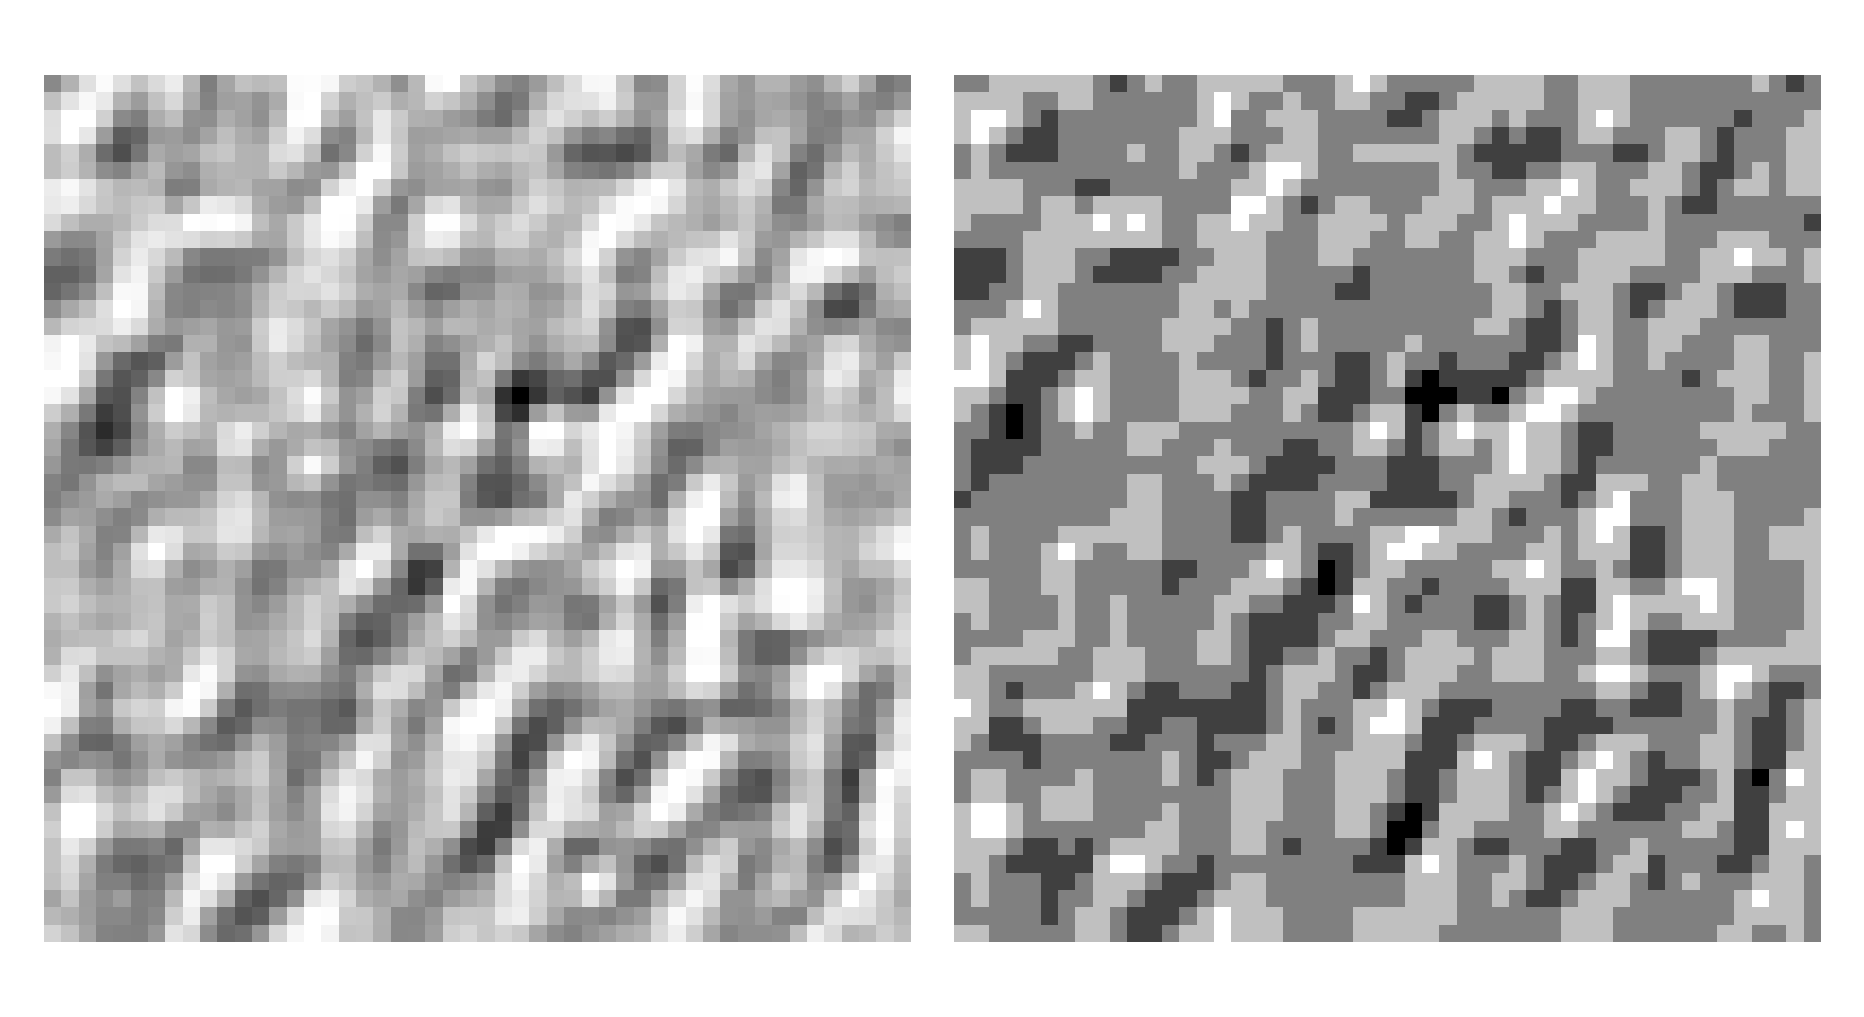
\includegraphics[width=0.9\textwidth]{./assets/roi-shallow.png}
    \caption{\label{fig:roi-shallow} Esempio di ROI estratta per algoritmo di shallow learning (sinistra) e
    di versione digitalizzata su 5 livelli di grigio per il calcolo di GLCM e GLRLM (destra).}
\end{figure}


Dalla GLRLM si estraggono ulteriori 11 valori statistici.
Infine, l'ultima trasformazione da applicare all'immagine è la traduzione in
dominio di frequenza tramite la {\it Discrete Fourier Transform} (DFT), da cui
si estraggono gli ultimi 3 valori statistici portando il totale a 32.
In tabella \ref{table:features-toma} il dettaglio dei valori statistici impiegati.

\begin{table}
        \center
        \begin{tabular}[h]{||c|c|c|c||}
            \hline 
            \textbf{Primo Ordine} & \textbf{GLCM} & \textbf{GLRLM} & \textbf{DFT} \\
            \hline 
            \hline 
            Media & Contrasto & GLN & Freq. Massima \\
            Mediana & Correlazione & GLNN & Banda \\
            10 Percentile & Energia & HGLRE & Freq. di Kurtosis \\
            90 Percentile & Omogeneità & LGLRE & \\
            Diff. Interquantile & & LRE & \\
            Media Quadratica & & LRHGLE & \\
            Dev. Standard & & LRLGE & \\
            Varianza & & MAD & \\
            Uniformità & & RLN & \\
            {\it Skewness} & & RLNN & \\
            & & RP & \\
            & & SRE & \\
            & & SRHGLE & \\
            & & SRLGLE & \\
            \hline 
        \end{tabular}
        \caption{\label{table:features-toma}Valori statistici estratti dalle ROI.}
    % \end{center}
\end{table}

I valori raccolti da ogni singola ROI vengono raccolti e normalizzati tramite
{\it min-max}. 
Indicando con $max(x,i)$ il valore massimo dell'$i$-esima componente
del vettore $\vec{x}$ presente nel nostro dataset, ed analogamente
per $min(x,i)$, si normalizzano i vettori ricavati da equazione \ref{eq:minmaxnorm}.

\begin{equation}\label{eq:minmaxnorm}
    \vec{x}_{norm} = \frac{\vec{x} - min(x,i)}{max(x,i) - min(x,i)}
\end{equation}

Questo viene fatto perché le varie componenti possono variare molto tra loro
in termini di magnitudine, e potrebbero quindi ingannare gli alberi
a credere che variando di più abbiano un significato maggiore e quindi una
maggiore rilevanza nella classificazione.\\
A differenza di quanto svolto inizialmente in \cite{Toma2022}, la divisione
dei campioni non viene effettuata a posteriori ma a priori:
inizialmente si raccoglievano tutti i campioni e si divdeva in tre parti,
{\it train}, {\it validation} e {\it test}, ma in questo caso si è deciso di optare
per una divisione iniziale delle immagini in questi tre set in modo che
il modello non possa avere indizi extra su una ROI che deve valutare
in fase di test basandosi su una somiglianza di una ROI adiacente o 
parzialmente sovrapposta cui ha avuto accesso in fase di train.

\begin{figure}[h]
    \center
    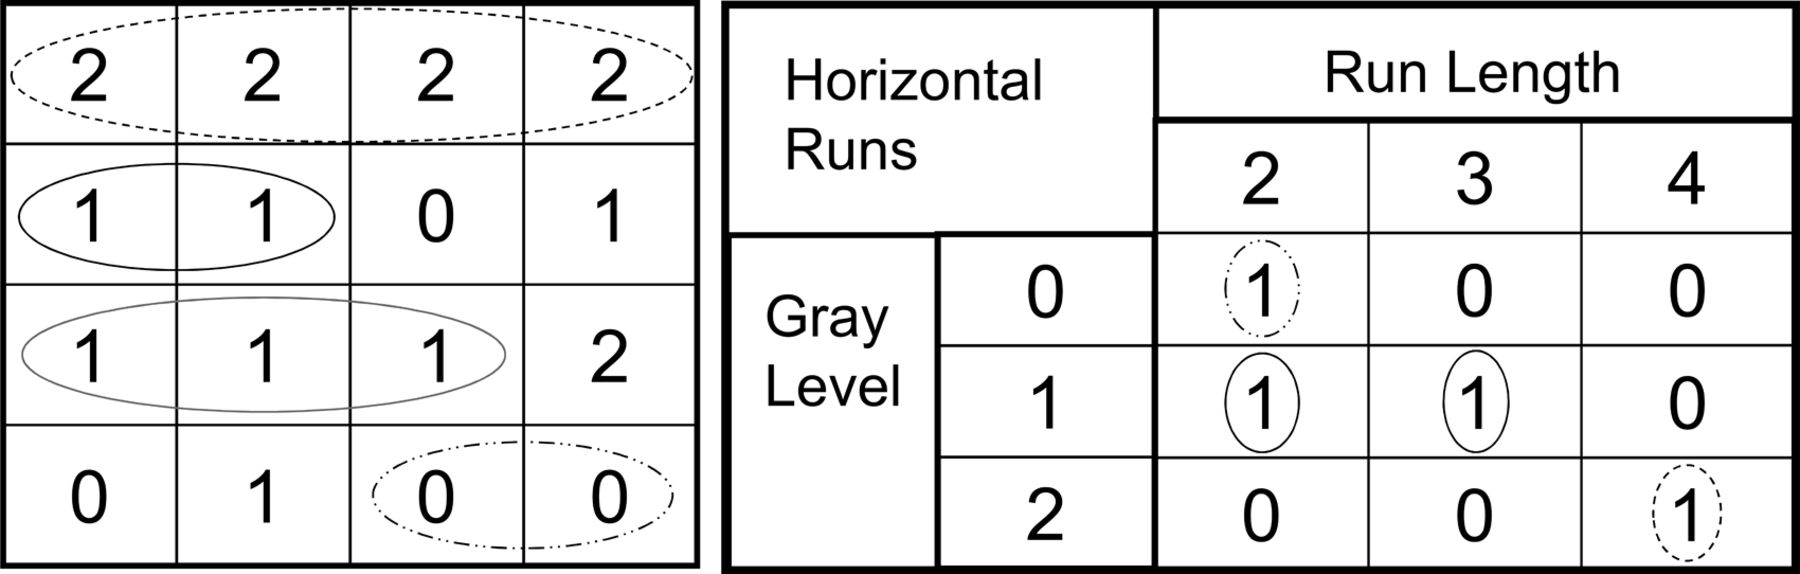
\includegraphics[width=0.9\textwidth]{./assets/glrlm.jpg}
    \caption{\label{fig:glrlm}Calcolo di una GLRLM a 3 livelli di grigio con angolo $\theta$ uguale a 0°, fonte: http://www.ajnr.org/content/36/7/1343/F2}
\end{figure}

A questo punto ogni ROI viene classificata e a partire da essa viene
costruita una maschera globale dell'immagine.
Visto che le ROI vengono estratte con una sovrapposizione spaziale del 40\%,
potremmo avere che alcuni pixel vengano classificati contemporaneeamente
come patologiche che come sane.
Per risolvere questo problema si è classificato il singolo pixel tramite
coefficiente di Dice con soglia impostata a 0.5, che si traduce
praticamente in una classificazione come appartente a una data classe
se la maggioranza delle classificazioni appartengono a quella data classe.
Vengono infine applicati degli operatori morfologi di chiusura, erosione e dilazione
per ottenere una maschera meglio formata.

\begin{figure}[h]
    \center
    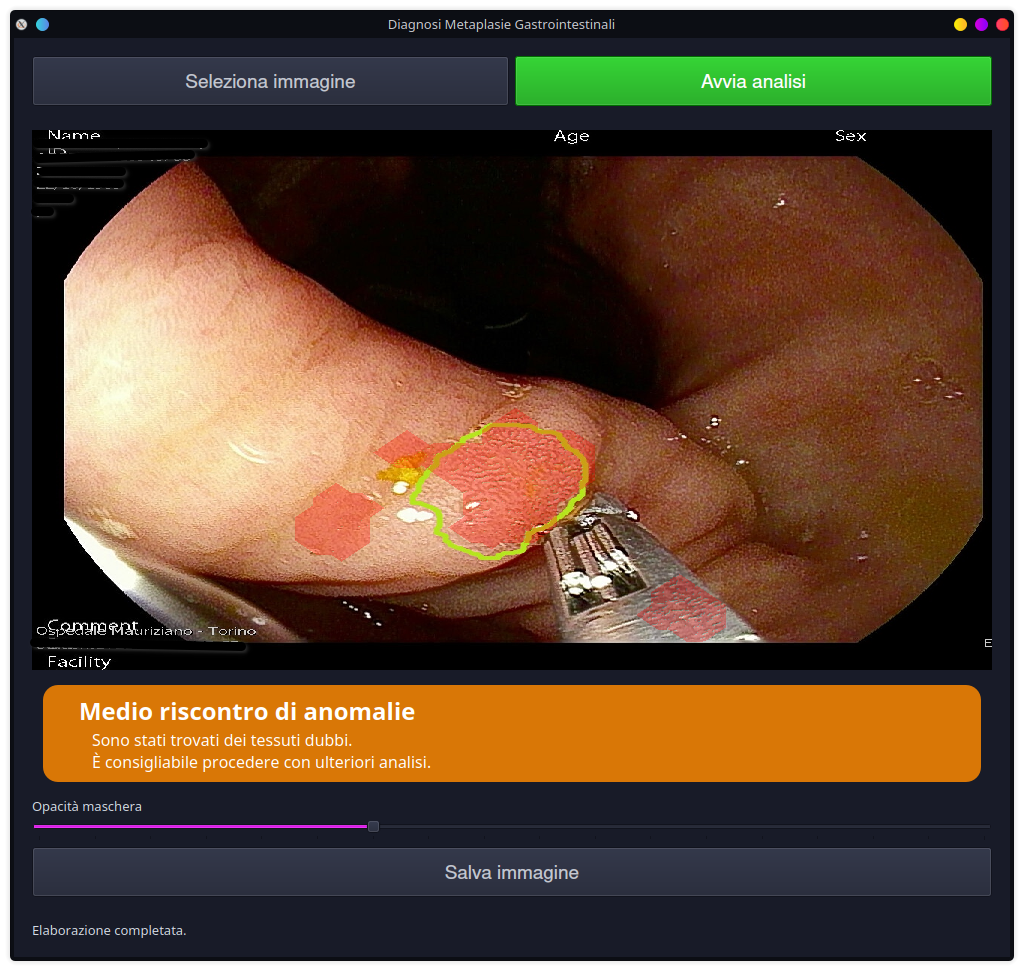
\includegraphics[width=0.9\textwidth]{./assets/gui-one.png}
    \caption{\label{fig:gui-one}Interfaccia grafica per la classificazione delle ROI. La zona cerchiata in verde indica l'area che desidereremmo rilevare, le zone a sovrapposizione rossa indicano le zone rilevate come anomale.}
\end{figure}

Presentata questa possibile implementazione abbiamo compreso le grosse
limitazioni che un approccio di questo genere ha.
Per iniziare possiamo notare delle prestazioni da parte del modello non
troppo soddisfacenti.
Una metrica molto utile per comprendere lo scontento è la precisione,
che indica il numero di predizioni corrette sul totale delle predizioni per ogni
classe.
Se quindi per la classe ritenuta sana abbiamo una precisione molto alta, lo stesso
non si puo' dire per quella patologica, che si ferma a circa il 50\%, un valore
troppo basso per un impiego reale.\\
Oltre i problemi di prestazioni, interloquendo con il personale medico
abbiamo idenfiticato ulteriori problemi di natura tecnica.
Il primo, visibile anche il foto, è che l'utilizzo dell'immagine in modalità
bianco e nero faccia perdere moltissime informazioni che potrebbero essere
fondamentali in fase di classificazione.
Ad esempio, come possibile vedere nella figura \ref{fig:gui-one}, un corpo
sicuramente esterno allo stomaco di colore grigio viene in parte
scambiato come tessuto patologico, cosa che difficilmente sarebbe accaduta
utilizzando una versione a colori dell'immagine.\\
Abbiamo poi che l'analisi delle immagini in un secondo momento non risulta
di grande utilità per il personale medico, che ha bisogno di avere un 
riscontro immediato durante l'endoscopia.
Va fatto notare che l'adattamento del modello a funzionare in tempo reale
su un video in input è una strada difficilmente percorribile, in quanto
una prima implementazione dell'algoritmo impiega circa 10 secondi per classificare
la singola immagine.
Quasi l'interità del tempo di elaborazione è speso nel calcolo delle
GLCM e delle GLRLM, dalla mole di calcolo discretamente elevata che aumenta
considerando il grande numero che se ne devono calcolare. \\

In ultimo, grazie al contributo del personale medico, è stato reso evidente
come il considerare le immagini estratte dai 3 filtri che l'I-SCAN utilizza
puo' essere potenzialmente controproducente.
Nello specifico, se nel processo di {\it shuffling}, per pura casualità,
si avesse che vi siano più immagini sane per un dato filtro che per un altro,
potrebbe erroneamente imparare a riconoscere la distribuzione delle
feature estratte da quelle ROI come meno probabilmente patologiche.

\subsection{\label{sec:deep-learning}Tecniche Deep Learning: Reti Neurali Convoluzionali}

Passiamo ora alla seconda possibilità che è stata valutata nello
sviluppo dell'applicativo, che riprende studi nel settore \cite{ilpaper}
che hanno dimostrato ottenere buoni risultati e fanno uso di reti neurali,
ovvero modelli di apprendimento profondo.
Questo significa che a differenza del precedente algoritmo non è possibile
comprendere il processo di classificazione, se non tramite interventi 
specifici all'architettura interna della rete, ma solitamente permettono
anche di ottenere risultati migliori, soprattutto nel caso di analisi di 
immagini in cui hanno sin da principio dimostrato una grossa dominanza 
sui modelli di apprendimento superficiale.

Un generico modello di {\it semantic segmentation} prevede varie
componenti e varie fasi.
Anzitutto il modello utilizza le immagini a colore e non convertite
in bianco e nero, e questo potrebbe dare grossi vantaggi rispetto
alla controparte di apprendimento superficiale.
La fase di {\it pre-processing} è sostanzialmente diversa non solo
nella realizzazione ma anche negli intenti:
se di fatto nell'algoritmo visto in \ref{sec:shallow-learning} lo
scopo era rendere i dati in input quanto più diferibili possibili,
qui invece si punta ad aggiungere disturbi ed alterazioni casuali per
due finalità:
la prima è quella di rendere il modello più generale e robusto,
e quindi più performante;
la seconda è per fini di {\it data-agumentation}, di cui 
parleremo più approfonditamente in \ref{sec:Dataset}.
A questo punto inizia la {\it feature extraction}, che consiste
nell'impiego di varie sequenze di filtri convoluzioni e di operatori
di {\it pooling}.
Il funzionamento generale di questi modelli è piramidale, dove si
esegue filtro $\to$ pooling $\to$ filtro $\to$ pooling $\to$ ...
come nella figura \ref{fig:cnn}, ma l'algoritmo specifico usa
un approccio leggermente diverso e verrà discusso nel dettaglio
in \ref{sec:bisenet}.
Lo scopo dei filtri è estrarre informazioni dall'immagine,
mentre quello degli strati di pooling e comprimere queste
informazioni che sarebbero altrimenti troppo numerose e dunque
intrattabili.

Infine dal risultato degli algoritmi di {\it region proposal}
identificano le zone di rilievo e su queste eseguono la classificazione.
È bene notare che anche questa fase è soggetta ad apprendimento,
ovvero il modello impara nel tempo a riconoscere ROI che potrebbero
essere interessanti o meno, e le zone dell'immagine che non
vengono estratte come ROI sono automaticamente classificate come
classe "sfondo", nel nostro caso "sano".
Inoltre a differenza dell'algoritmo visto in \ref{sec:shallow-learning}
il numero e la dimensione delle ROI estratte non è fisso.


\begin{figure}[ht]
    \centering
    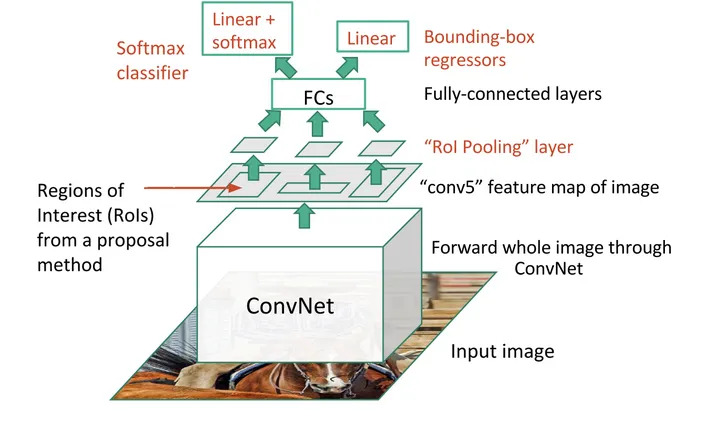
\includegraphics[width=0.9\textwidth]{./assets/cnn.jpg}
    \caption{\label{fig:cnn}Visualizzazione del processo di classificazione di un'immagine. Fonte: https://towardsdatascience.com/region-of-interest-pooling-f7c637f409af}
\end{figure}

Le ROI estratte sono quindi sottoposte a una testa, detto livello
completamente connesso, che etichetta ogni singolo pixel al suo
interno.
È quindi evidente che in questo caso il modello ha il compito,
oltre quello di riconoscere se la ROI sia potenzialemente patologica
o meno, anche di riconoscere quale parte della ROI lo è, e dunque
a livello globale debba apprendere non solo a riconoscere le zone
anomale ma anche a tracciarne la maschera.

\subsection{\label{sec:bisenet}Algoritmo II}

Capito il funzionamento di un generico modello di
{\it semantic segmentation}, seppure ogni architettura sia poi
possa avere nel merito differenze più o meno significative,
possiamo andare a vedere nel dettaglio quella scelta per 
questo specifico caso, ovvero la rete BiseNet \cite{bisenet}.

{\it BiSeNet}\cite{bisenet}, acronimo di
{\it Bilateral Segmentation Network}, prende il nome per via
della sua architettura interna che si dirama in due parti.
Come discusso in precedenza la caratteristica fondamentale
delle reti neurali che le rende così accurate nel riconoscere
le immagini è la fase di estrazione delle {\it features} che avviene
tramite filtri convoluzionali e pooling.
Un filtro convoluzionale puo' avere varie caratteristiche,
tra cui la sua dimensione, la sua profondità, il suo {\it stride},
ovvero quanto si sposta in orizzontale o in verticale ad ogni
iterazione, e la sua {\it padding}, ovvero se si aggiungono
zeri intorno all'immagine per farla avere dimensioni multipli
della dimensione del filtro, ma soprattuo il numero di filtri da
applicare.
In linea generale si ha che con un numero più elevato di filtri
le prestazioni siano migliori, ma anche che il processo
sia più pesante computazionalmente parlando e dunque più
lento, cosa che va tenuta in considerazione nel momento in cui 
si tenti, come nel nostro caso, di realizzare un sistema che funzioni
in tempo reale.


\begin{figure}
    \center
    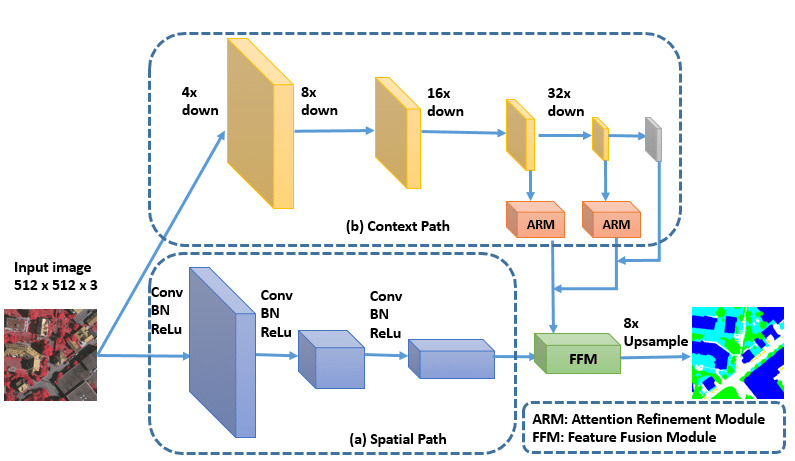
\includegraphics[width=0.9\textwidth]{./assets/bisenet.jpg}
    \caption{\label{fig:bisenet}Visualizzazione ad alto livello dell'architettura di BiSeNet. Fonte: researchgate.net}
\end{figure}

In letteratura si ha che per architetture più veloci, che tentano
di raccogliere più informazioni di alto livello a scapito di quelle
specifiche e locali, si utilizzino tali filtri in maniera ridotta,
preferendo la codifica delle informazioni tramite l'uso più esteso
di livelli di pooling, mentre in contesti in cui si cerca di
cogliere in maniera più fine i dettagli si utilizzino di più i filtri.
BiSeNet tenta di fondere i due approcci, utilizzando un primo ramo
che è chiamato {\it context path} (CP) e che si occupa di estrarre
informazioni di alto livello, e un secondo ramo che è chiamato
{\it spatial path} (SP) e che si occupa invece di estrarre informazioni
di basso livello, utilizzando le tecniche detto per ora.
Infine i due rami vengono uniti tramite dei
{\it feature fusion module} (FFM) e degli
{\it attention refinement module}.
Il secondo si occupa di unire più stadi della CP al fine di ottenerne
uno finale più accurato, tramite dei meccanismi di attenzione che sono
una tecnica auto-supervisione dei modelli per apprendere quali 
informazioni tra quelle estratte siano più rilevanti di altre,
mentre il primo esegue varie operazioni matematiche tra i due
risultati, tipo la somma o il prodotto componente per componente, 
in modo da ottenre un unico risultato finale.
Questo risultato viene infine valutato e ridimensionato in modo
da ottenere una dimensione pari a quella in ingresso.



\section{\label{sec:Dataset}Dataset}

Allenando un modello di intelligenza artificiale è necessario
rifelttere sul tipo di dati che si vogliono utilizzare per
l'apprendimento.
Nel mondo accademico sono disponibili vari dataset che vengono
considerati come banco di prova nel momento in cui si vuole
produrre un nuovo tipo di modello, ma spesso tali dati non 
sono invece adatti se si sa già quale modello si intende
utilizzare e si vuole invece creare qualcosa di concretamente
utilizzabile, ed è quindi necessario raccogliere o ottenre
i dati necessari in altri modi.
Tuttavia, come nel nostro caso, questi dataset possono comunque
essere messi a supporto dei nostri dati specifici.

Per l'allenamento del modello per il nostro applicativo faremo
uso di due dataset, uno pubblico ed uno creato {\it ad-hoc}
dall'Ospedale Mauriziano di Torino.
Il primo è il dataset HyperKvasir\ref{tab:hyperkvasir},
che raccoglie una moltitutine di dati riguardante
vari riscontri patologici di più parti intestinali, assieme
anche a dei video.
Una criticità di questo dataset è che, seppur di grandi dimensioni,
non contiene dati di nostro diretto interesse.
L'altro dataset è invece composto da acquisizioni endoscopiche
svolte dal personale medico dell'ospedale Mauriziano di Torino,
che invece raffigura esattamente il nostro caso di interesse.
Nel suo caso, la criticità è la scarsa quantità di dati
a disposizione.
Se infatti sono state messe a disposizione ben 1194 immagini,
i riscontri patologici, di fondamentale importanza in quanto
è solo in base ad essi che il modello puo' imparare a discriminare
tra i tessuti sani e quelli patologici, sono solo 49.
A peggiorare la situazione è il fatto che di queste 49 immagini
solo 38 sono annotate ed utilizzabili, dove per annotate
si intende l'indicazione dell'area patologica di interesse, e per
utilizzabili che si disponga sia dell'immagine originale che di
quella non annotata.

Per questi motivi, nello sviluppo dell'algoritmo descritto in
\ref{sec:shallow-learning} si è utilizzato il solo dataset
Mauriziano, mentre per il modello di deep learning
descritto in \ref{sec:deep-learning} è stato necessario
l'utilizzo del dataset HyperKvasir.

\subsection{\label{sec:mauriziano}Dataset Mauriziano}

A differenza dei modelli di deep learning, gli alberi decisionali
di cui in \ref{sec:shallow-learning} non operano direttamene
con le immagini, ma con vettori di dati che descrivano a livello
statistico le nostre immagini.
In questa sezione discuteremo il modo in cui questa trasformazione
viene eseguita.

Il puntodi partenza sono le immagini stesse, e a differenza di
quanto accade per il modello descritto in \ref{sec:deep-learning},
utilizzare le immagini contenenti l'annotazione non dà una
quantità eccessiva di informazioni per la predizione, quindi
potremo utilizzare tutte e 49 le immagini patologiche.
Inoltre il modello puo' comunque giovare dall'avere a disposizione
anche delle immagini sane per allenarsi. Per questo motivo verrano
utilizate anche 25 immagini sane, meno di quelle patologiche per
non creare eccessivo scompenso.

\begin{figure}
    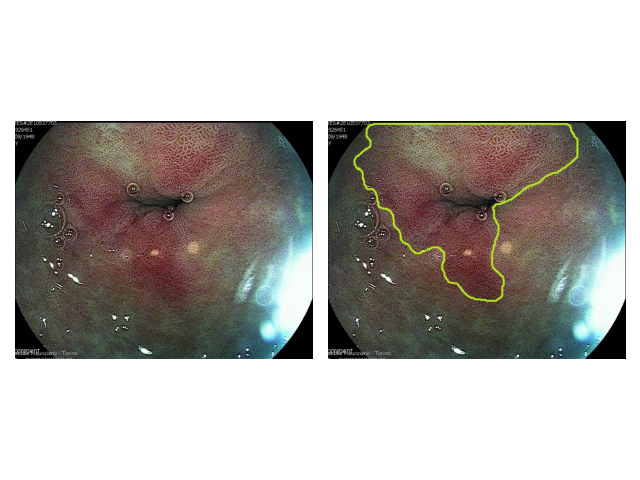
\includegraphics[width=0.9\textwidth]{./assets/side-by-side.png}
    \caption{\label{fig:side-by-side}Esempio di immagine originale (sinistra) e
    di immagine con annotazione {\it hard-coded} (destra)}
\end{figure}

Come discusso, le immagini si presentano come immagini {\it hard-coded}.
Questo significa che l'annotazione di dove il tessuto si trovi
nell'immagine è stata eseguita in maniera irreversibile sull'immagine,
e non è direttamente utilizzabile per l'apprendimento.
Tagliate via alcune porzioni superflue, come la seconda visuale che
non è di nostro interesse, e tagliando via i dati sensibili del paziente,
il primo step è dunque andare a ottenere una rappresentazione più
fruibile dell'annotazione.


Partendo da una maschera vuota, è possibile sfruttare il colore
verde acceso dell'annotazione, visibile nell'immagine \ref{fig:side-by-side}
per identificare un anello che racchiuda l'annotazione.
A questo anello si applica poi un operatore morfologico di dilatazione,
per assicurarsi che tale anello sia chiuso e non ci siano buchi lungo la
sua traccia.
A questo punto si applica un secondo operatore morfologico, questa
volta di chiusura, in modo da andare a riempire la traccia e ottenere
una maschera uniforme lungo tutto l'area patolgica, e si termina
con un'operatore morfolico di erosione per annullare gli effetti della
precedente dilatazione.
A questo punto abbiamo ottenuto la maschera di annotazione da
usare con la nostra immagine non annotata, che deve essere
salvata in un formato che possa essere compresso senza perdita.
In questo caso si è scelto di utilizzare per il modello di 
{\it shallow learning} il formato {\it NPY}, che permette di salvare
e leggere direttamente la matrice di pixel tramite apposite
librerie Python, e per quello di {\it deep learning} il formato
{\it PNG} che è quello impiegato dalla libreria Pytorch per
elaborare le annotazioni.


\begin{figure}[h]
    \center
    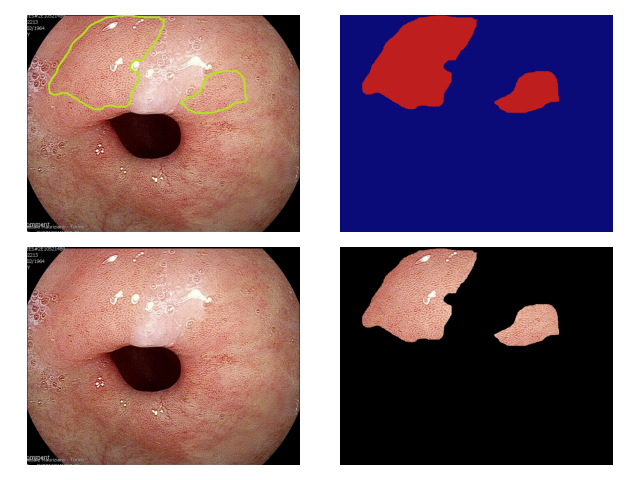
\includegraphics[width=0.9\textwidth]{./assets/cutout2.png}
    \caption{\label{fig:cutout}Processo di estrazione delle maschere.
    In senso orario: immagine annotata, maschera calcolata, immagine originale,
    ipotetico ritaglio della sola parte patologica.}
\end{figure}

Le immagini vengono poi processate per poter essere elaborate
dall'algoritmo, come descritto in \ref{sec:shallow-learning}.
Si prosegue poi andando a trasformare le immagini in
{\it Region of Interest} (ROI), ovvero piccole sezioni di immagine
di dimensione fissa 50$\times$50 pixel, con una sovrapposizione
del 40\% tra una ROI e la successiva in entrambe le direzioni,
ovvero di 20 pixel.
In fase di estrazione vengono filtrate via le ROI che non contengano
effettivamnte del tessuto andando a scartare quelle che siano
composte per più del 70\% da pixel neri, e viene confrontata
la posizione da dove è estratta la ROI con la corrispondente
posizione nella maschera: nel caso in cui oltre il 50\% della ROI
ricada in una zona patologica, essa viene classificata come ROI
patologica, altrimenti essa viene classificata come ROI sana.

\begin{figure}
    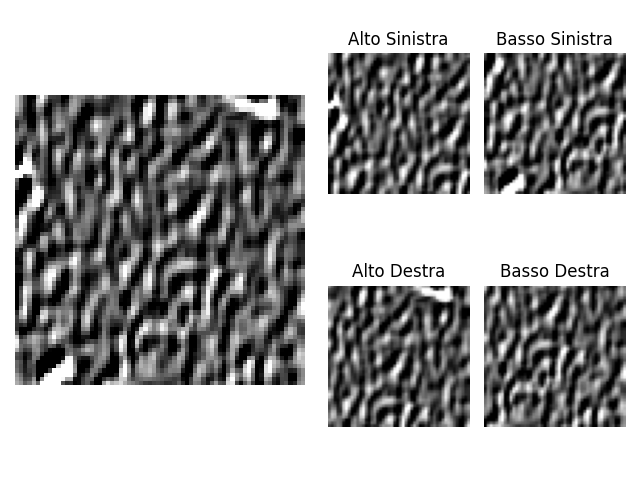
\includegraphics[width=\textwidth]{./assets/path-overlap.png}
    \caption{\label{fig:patch-overlap}Esempio di sovrapposizione delle ROI}
\end{figure}

Appare evidente che essendo le zone di tessuto patoligico solo
una piccola parte dell'immagine e utilizzando anche immagini
totalmente sane, il numero di ROI sane sia molto più alto di
quelle patologiche: per questo motivo le ROI patologiche
vengono salvate anche rotate di 90° in senso orario e salvate
nuovamente, in modo da aumentare la quantità di dati
a disposizione.
Estratte le ROI, esse vengono processate come descritto in
\ref{sec:shallow-learning} e i dati vengono salvati
in un file di formato {\it CSV}, assieme ai valori massimi
e minimi di ogni {\it feature} che servirà poi per eseguire
la normalizzazione.
Un sommaario dei dati estratti è riportato nella tabella
\ref{tab:mauriziano}.
In fase di allenamento del modello il 10\% delle
{\it features} di train viene utilizzato come
dataset di validazione per monitorare l'andamento.

\begin{table}
    \center
    \begin{tabular}[h]{||c||c|c|c||}
        \hline
        & Train & Test & Totale \\
        \hline
        Immagini Sane & 20 & 5 & 25 \\
        \hline
        Imagini Patologiche & 40 & 9 & 49 \\
        \hline
        ROI Sane & 93.757 & 22.739 & 116.469 \\
        \hline
        ROI Patologiche & 52.840 & 11.602 & 64.442 \\
        \hline
        \hline
        \multirow{2}{*}{Totale} & 60 & 13 & 73 \\ \cline{2-4}
        & 146'597 & 34.341 & 180.938 \\
        \hline
    \end{tabular}
    \caption{\label{tab:mauriziano}Composizione del dataset Mauriziano per
    algoritmo di Shallow Learning}
\end{table}

Nel caso dell'algoritmo descritto in \ref{sec:deep-learning},
è sufficiente avere le maschere di annotazione, ma è richiesto
che l'immagine utilizzata in ingresso sia pulita e senza annotazioni.
Come già discusso però, il numero esiguo di campioni lo rende
inutilizzabile da solo per l'allenamento di un modello di
{\it deep learning}, o almeno non uno di cui i risultati abbiano
una qualche rilevanza statistica.
Le 49 immagini patologiche vengono quindi divise in maniera poco
generosa verso la porzione dedicata al training, divsione
descritta nella tabella \ref{tab:mauriziano-ii}, in quanto questa
verrà utilizzata solo in fase di {\it fine-tuning} del modello,
mentre il resto viene diviso in maniera equa tra validazione e test.
Infine, usando il software {\tt ffmpeg} tute le immagini vengono
usate per creare un video da utilizzare in fase di dimostrazione
dell'applicativo.
Solitamente non è corretto utilizzare immagini impiegate in fase
di validazione o di allenamento per testare un modello,
tuttavia non andando a valutare le prestazioni su tale video
ma solo la funzionalità questo comportamento risulta accettabile.
Il video in questione viene impostato per avere un {\it frame-rate}
10 FPS non per vincoli tecnici del modello ma per poter
essere apprezzato dall'occhio umano.

\begin{table}
    \center
    \begin{tabular}[h]{||c|c||}
        \hline
        Split & Immagini \\
        \hline
        Train & ? \\
        Test & ? \\
        Validation & ? \\
        \hline
        Totale & 49 \\
        \hline
    \end{tabular}
    \caption{\label{tab:mauriziano-ii}Divisione del dataset Mauriziano per
    algoritmo di Deep Learning}
\end{table}



\subsection{Il Dataset HyperKvasir}

Il dataset HyperKvaris\cite{HyperKvasirDataset} nasce per sopperire
alla mancanza di dati medici per lo studio e l'addestramento
di modelli di intelligenza artificiale.
La raccolta di dati è, in ogni ambito, un lavoro costoso non 
soltatno in termini monetari ma spesso e volentieri anche
per fattori di tempo e di risorse umane.
Dataset comunemente usati nella ricerca di modelli di intelligenza
artificiale, come {\it Common Object and Context}\cite{cocodataset}
(COCO) ed {\it ImageNet} \cite{imagenet} contengono
immagini di oggetti comuni presi dalla quotidianità,
quindi classificabili da qualunque persona: ciò non toglie
che il processo di annotazione, che puo' prendere
varie forme come la classificazione, la segmentazione e la
circoscrizione, sia un processo lungo e ripetitivo.

Nel caso specifico della medicina, le cose si complicano
molto di più.
Sin dal principio, è molto diffile ottenere i dati grezzi,
quindi non annotati, spesso anche per tutelare la privacy
del paziente stesso, o comunque è difficile ottenerne in
quantità sufficienti, ed anche quando questo accade
è necessario l'impiego di personale medico altamente
specializzato, nel nostro caso nel settore della
gastroenterologia, per annotare e segmentare le immagini.
Specificiatamente per l'ambito medico, è anche preferibile
avere più di un riscontro.

HyperKvasir è dunque la più grande raccolta di immagini
e video di esami di endoscopia digestiva, rilasciato proprio
allo scopo di facilitare la ricerca in questo ambito.
Va fatto tuttavia notare che quanto detto in precedenza resta
purtroppo vero:
non lasciandoci trarre in inganno dalla dimensione del dataset,
che ammonta a ben 110'00' immagini e 374 video, bisogna
constatare che si tratti comunque di un dataset molto
eterogeno nella sua composizione.
Delle 110'000 immagini, infatti, 99'000 sono che sono
talmente prive di annotazioni, vale a dire nè classificate
nè segmentate in alcun modo, e delle restanti 11'000
solo 1'000 sono immagini di cui sono disponibili
le annotazioni di segmentazione.
Per ultimo, trattandosi di un dataset per lo studio
di analisi endoscopiche, le immagini riportanti metaplasie
sono presenti solo come immagini classificate ma non come
segmentate, fattore che renderebbe impraticabile
l'utilizzo del nostro modello.

\begin{table}
    \center
    \begin{tabular}{||c|c|c|c||}
        \hline
        Tipologia & \# Campioni & \# Classi & Dimensione (MB) \\
        \hline
        \hline
        Classificate & 10'662 & 23 & 3'960 \\
        \hline
        Segmentate & 1'000 & 1 (Polyp) & 57 \\
        \hline
        Non annotate & 99'417 & 0 & 29'940 \\
        \hline
        Video & 374 & 30 & 32'539 \\
        \hline
        \hline
        Totale & 111'453 & --- & 66'496 \\
        \hline
    \end{tabular}
    \caption{\label{tab:hyperkvasir}Composizione del dataset HyperKvasir}
\end{table}

È ovviamente improprio l'utilizzo di un dataset che raffiguri
oggetti diversi da quelli che si possono riscontrare nel 
contesto di applicazione per l'addestramento del modello,
tuttavia avendo a che fare con un numero di campioni
relativo ad esso molto limitato si è scelto di utilizzarlo
in congiunzione con il dataset descritto in \ref{sec:dataset-mauriziano}.
Questo è possibile tramite l'impiego del {\it transfer learning},
che consiste nell'usare come base di partenza per l'addestramento
di un nuovo modello uno già allenato su un dataset con
caratteristiche simili al nuovo.
Questa tecnica è generalmente utilizzata per velocizzare
il processo di apprendimento, insieme anche al raggiungimento
di risultati migliori, ma è anche molto utile quando si 
dispone di pochi dati, come nel nostro caso.
È bene notare dunque che l'impiego di {\it transfer learning}
per lo sviluppo di modelli di intelligenza artificiale non è
dunque un ultima risorsa ma bensì la norma, vista la
pervasività che ha dimostrato nei vari ambiti di applicazione.

In ultimo, il dataset HyperKvasir è anche molto eterogeno
nella forma in cui si presentano le immagini.
A differenza del dataset in \ref{sec:dataset-mauriziano} infatti,
dove le acquisizioni sono state effettuate tutte con la medesima
macchina, sono di uguale ed altissima risoluzione, nel caso
di HyperKvasir infatti abbiamo con immagini provenienti da diverse
fonti e di qualità generalmente inferiore.

%% \begin{table}
    %% \center
    %% \begin{tabular}{||c|c|c|c|c||}
        %% \hline
        %% & W < 400 & 400 < W < 600 & 600 < W < 800 & W > 800 \\ 
        %% \hline
        %% H < 400 &  &  &  & \\ 
        %% \hline
        %% 400 < H < 800 &  &  &  & \\ 
        %% \hline
        %% 600 < H < 800  &  &  &  & \\ 
        %% \hline
        %% H > 800 & &  &  & \\ 
        %% \hline
    %% \end{tabular}
%% \end{table}

\section{Processi}
\subsection{La Libreria MMSegmentation}
\subsection{Allenamento del Modello}
\subsection{Valutazione del Modello}